% $Id$

%\section{Object Model}

In Figure 5, we see how a ESM component's clock checks its alarms.  After
the clock's current time is incremented (Model time stepped), the clock checks
all its alarms to see if its time for them to start or stop ringing.  All the
user needs to know is how to initialize the alarms and time step the clock;
the alarm checking happens internally "under the hood."
   
\begin{center}
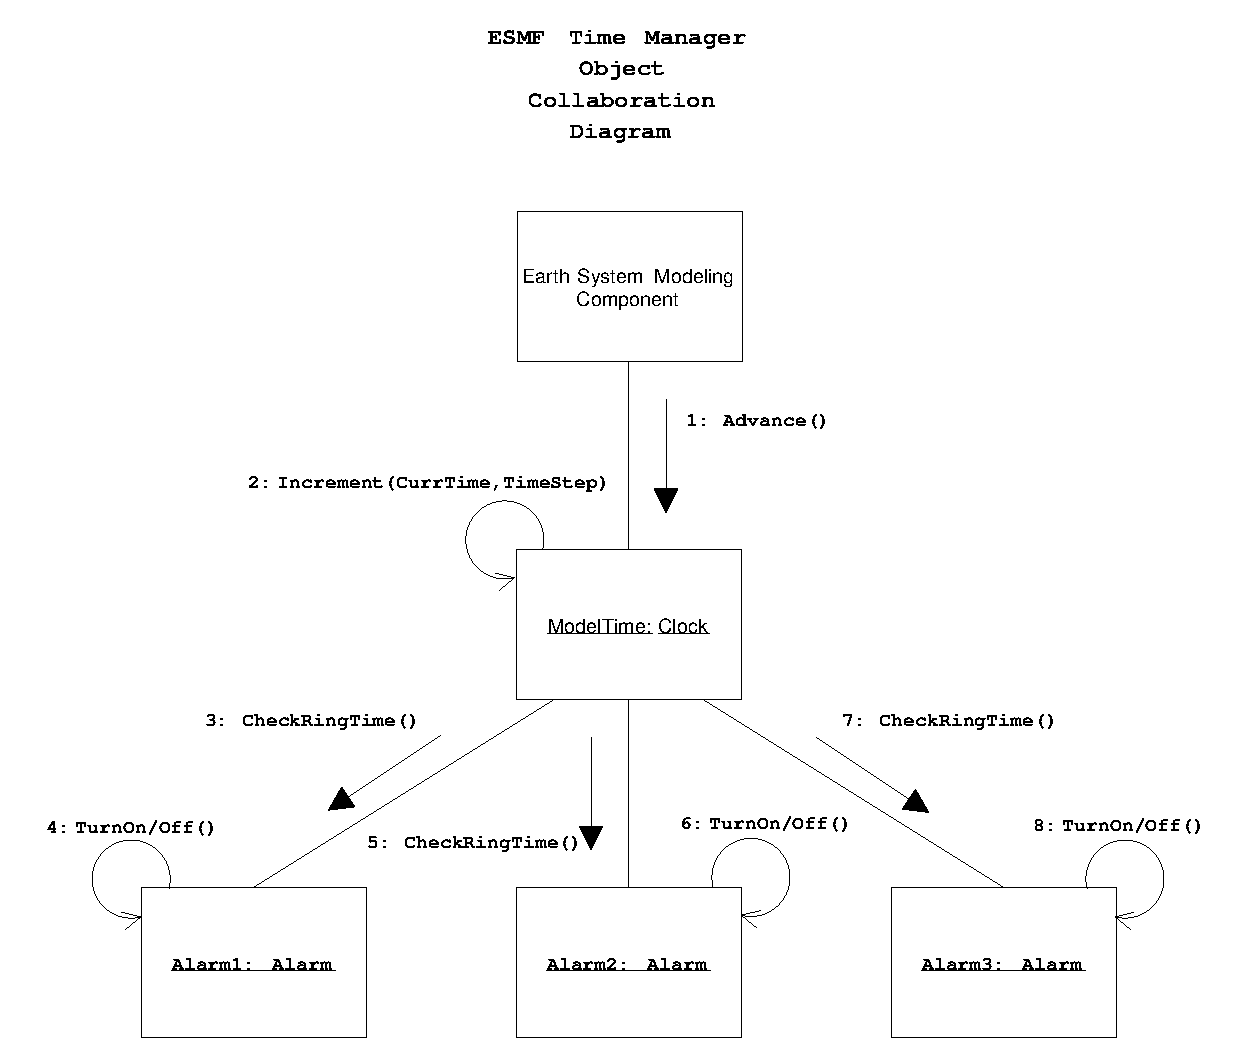
\includegraphics{TimeMgrOCD3.EPS}
   
Figure 5.  ESMF Time Manager Check Alarms Scenario
   
\end{center}
